\section{Analisi della dipendenza tra le variabili}


\subsection{Analisi di correlazione}

\begin{figure}[H]
	\centering
	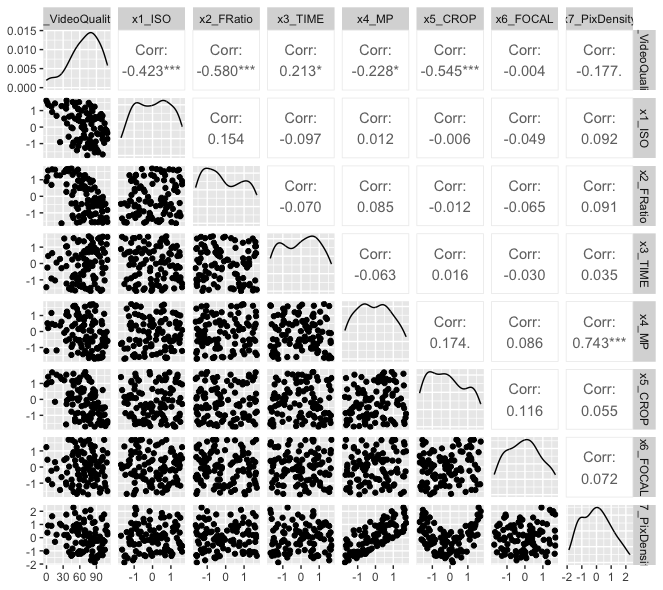
\includegraphics[width=0.90\textwidth]{../graphs/DescriptiveStatisticPlots/ggplot}
	\caption{Scatter plot delle variabili presenti nel dataset.}
\end{figure}

Dalla Figura (3) notiamo, anche dal coefficiente di correlazione, una dipendenza lineare tra le variabili:
\begin{itemize}
	\item \textbf{x4\_MP} e \textbf{x7\_PixDensity}
\end{itemize}
Invece notiamo la presenza di dipendenze non lineari che non vengono descritte dal coefficiente di correlazione. In particolare la notiamo tra le variabili:
\begin{itemize}
	\item \textbf{y\_VideoQuality} e \textbf{x1\_ISO}
	\item \textbf{y\_VideoQuality} e \textbf{x2\_FRatio}
	\item \textbf{y\_VideoQuality} e \textbf{x3\_Time}
	\item \textbf{y\_VideoQuality} e \textbf{x5\_CROP}
	\item \textbf{x5\_CROP} e \textbf{x7\_PixDensity}
\end{itemize}

\subsection{Analisi di regressione}
Le dipendenze tra la variabile y\_VideoQuality e le diverse variabili indipendenti sono state analizzate attraverso una regressione semplice sulle singole variabili indipendenti.
\begin{table}[H]
	\centering
	\begin{tabular}{|c|c|}
		\hline
		\textbf{Variabile indipendente} & \textbf{p-value} \\
		\hline
		x1\_ISO & $1.17e-05$ \\
		\hline
		x2\_FRatio & $2.63e-10$ \\ 
		\hline
		x3\_TIME & $0.0331e$ \\
		\hline
		x4\_MP & $0.0227$ \\
		\hline
		x5\_CROP & $4.39e-09$ \\
		\hline
		x6\_FOCAL & $0.97$ \\
		\hline
		x7\_PixDensity & $0.0775$ \\
		\hline
	\end{tabular}
	\caption{Sono rappresentati i p-value relativi alle regressioni delle singole variabili indipendenti al primo grado.}
	\label{tab:}
\end{table}
Diversamente da quanto ottenuto nell'analisi di correlazione, dalla Tabella (1) risultano rilevanti i regressori x1, x2, x3, x5. La stessa analisi è stata poi effettuata considerando anche i regressori al secondo ordine.

\begin{table}[H]
	\centering
	\begin{tabular}{|c|c|}
		\hline
		\textbf{Variabile indipendente} & \textbf{p-value} \\
		\hline
		x1\_ISO & $2.46e-03$ \\
		\hline
		x2\_FRatio & $1.28e-3$ \\ 
		\hline
		x3\_TIME & $0.3094$ \\
		\hline
		x4\_MP & $0.2899$ \\
		\hline
		x5\_CROP & $0.368$ \\
		\hline
		x6\_FOCAL & $0.770$ \\
		\hline
		x7\_PixDensity & $0.8038$ \\
		\hline
	\end{tabular}
	\caption{Sono rappresentati i p-value relativi alle regressioni delle singole variabili indipendenti al secondo grado.}
	\label{tab:}
\end{table}
Dalla Tabella (2) risulta evidente una dipendenza quadratica della variabile dipendente dai regressori x1, x2.

